\documentclass[aspectratio=169]{beamer}
\usepackage{ITMOtheme}

% Подключите этот пакет, чтобы использовать русский язык.
%\usepackage[english,russian]{babel}

% Если будет предупреждение "Package hyperref Warning: Glyph not defined in PD1 encoding"
%\hypersetup{unicode=true}


%Use this package to automatically format references.
\usepackage[style=mla]{biblatex}
\addbibresource{references.bib}


\titlegraphic{
\includegraphics[scale=.8]{itmo_logo_en_vert_blue.pdf}}
%\titlegraphic{
\includegraphics[scale=.8]{itmo_logo_rus_vert_blue.pdf}}

% use \title[short title]{full title}
\title[ITMO LaTex]{ITMO University LaTex Presentation}

%\subtitle[short subtitle]{long subtitle}

\author[Zabashta A.]{Alexey Zabashta}

%\institute[short institute]{long institute}

\where{ITMO University, St. Petersburg, Russia}
\date{\today}

%I don’t know if this affects anything.
\subject{example}
\keywords{ITMO University, LaTex teamplate, beamer}


\begin{document}

\begin{frame}[plain]
    \titlepage
\end{frame}


% You can use custom title, if you want.
%\begin{frame}[plain]
%	\itmopolygons{
%	\vfill
%		\includegraphics[height=0.2\paperheight]{itmo_white_rus.png}
%	\vfill
%		\usebeamerfont{title}{  \inserttitle\par} 
%	\vfill
%		\usebeamerfont{subtitle}{\insertsubtitle\par}
%	\vfill
%		\insertauthor\par
%	\vfill
%		\insertinstitute\par
%	\vfill
%		\insertplace  \;  \insertdate
%}
%\end{frame}



\begin{frame}{Outline}
 \tableofcontents
\end{frame}



\begin{frame}{Footcite and Footnote}

You can use \textbackslash footcite command to automatically formatted citation. For example\footcite{kopka1995guide}.

Or you can use \textbackslash footnote command for manual formatting or another footnote\footnote{Some text in a footnote.}.
\end{frame}



\section{First Section}

\subsection{Subsection Example} 

\begin{frame}
\frametitle{Paragraphs of Text}
Lorem ipsum dolor sit amet, consectetur adipiscing elit, sed do eiusmod tempor incididunt ut labore et dolore magna aliqua. Ut enim ad minim veniam, quis nostrud exercitation ullamco laboris nisi ut aliquip ex ea commodo consequat. Duis aute irure dolor in reprehenderit in voluptate velit esse cillum dolore eu fugiat nulla pariatur. Excepteur sint occaecat cupidatat non proident, sunt in culpa qui officia deserunt mollit anim id est laborum.

\alert{This text does not make any sense!}

\end{frame}


\section{Second Section} 

\begin{frame}
\frametitle{Blocks of Highlighted Text}
\begin{block}{Regular Block}
Lorem ipsum dolor sit amet, consectetur adipiscing elit. Integer lectus nisl, ultricies in feugiat rutrum, porttitor sit amet augue. Aliquam ut tortor mauris. Sed volutpat ante purus, quis accumsan dolor.
\end{block}

\begin{exampleblock}{Example Block}
Pellentesque sed tellus purus. Class aptent taciti sociosqu ad litora torquent per conubia nostra, per inceptos himenaeos. Vestibulum quis magna at risus dictum tempor eu vitae velit.
\end{exampleblock}

\begin{alertblock}{Alert Block}
Suspendisse tincidunt sagittis gravida. Curabitur condimentum, enim sed venenatis rutrum, ipsum neque consectetur orci, sed blandit justo nisi ac lacus.
\end{alertblock}
\end{frame}


\begin{frame}
\frametitle{Colors}

You can use main official predefined colors 
\textcolor{ITMOblue}{ITMOblue} and \textcolor{ITMOred}{ITMOred}, and also
 \textcolor{ITMOorange}{ITMOorange}, \textcolor{ITMOsky}{ITMOsky}, \textcolor{ITMOpistachio}{ITMOpistachio}, \textcolor{ITMOaqua}{ITMOaqua}, \textcolor{ITMOice}{ITMOice}, \textcolor{ITMOgold}{ITMOgold}, \textcolor{ITMOyellow}{ITMOyellow}, \textcolor{ITMOtomato}{ITMOtomato}, \textcolor{ITMOgreen}{ITMOgreen}.

\end{frame}



\subsection{Using columns}


\begin{frame}
\frametitle{Multiple Columns}
\begin{columns}[c] 

\column{.45\textwidth}{
    \begin{enumerate}
        \item First item
        \item Second item
        \item Third item
    \end{enumerate}
}

\column{.45\textwidth}{
    \begin{itemize}
        \item Some item
        \item Another item
        \item Also item
    \end{itemize}
}

\end{columns}
\end{frame}



\section{Other LaTex stuff}

\subsection{Tables}


\begin{frame}
\frametitle{Table}
\begin{table}[H] 
% Russian style caption
%\caption{Multiplication table of complex numbers}
\begin{tabular}{r | r r r r r} 
$a \times b$ & $0$ &  $1$ &  $i$ & $-1$ & $-i$ \\ \hline
         $0$ & $0$ &  $0$ &  $0$ &  $0$ &  $0$ \\
         $1$ & $0$ &  $1$ &  $i$ & $-1$ & $-i$ \\
         $i$ & $0$ &  $i$ & $-1$ & $-i$ &  $1$ \\
        $-1$ & $0$ & $-1$ & $-i$ &  $1$ &  $i$ \\
        $-i$ & $0$ & $-i$ &  $1$ &  $i$ & $-1$ \\
\end{tabular}
\caption{Multiplication table of complex numbers}
\end{table}
\end{frame}


\subsection{Theorems and Equations}


\begin{frame}
\frametitle{Theorem}
\begin{theorem}[Fermat's Last Theorem]
\begin{equation}
    \forall n, x, y, z \in \mathbb{N}: n > 2 \Rightarrow x^n + y^n \neq z^n
\end{equation}
\end{theorem}
I have discovered a truly remarkable proof of this theorem which this frame is too small to contain.
\end{frame}


\subsection{Figures}

\begin{frame}
\frametitle{Figure example}
\begin{figure}
    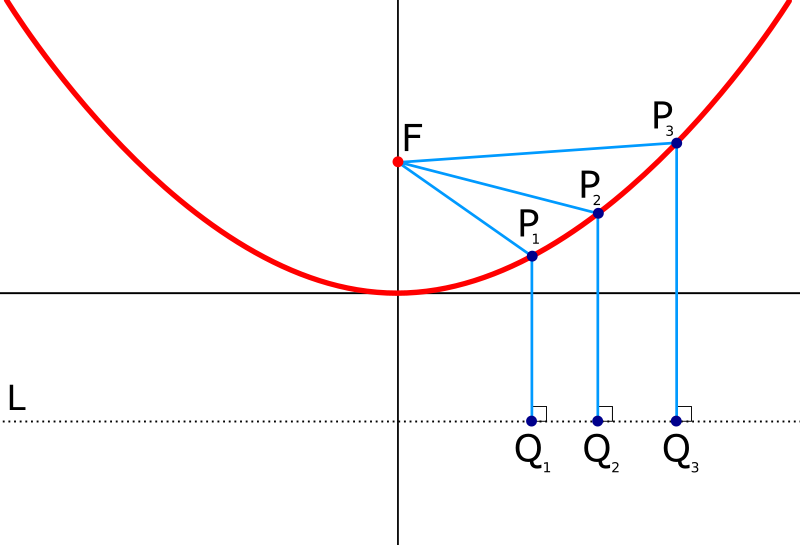
\includegraphics[scale=.3]{fig/parabola.png}
    \caption{Parabola with focus and directrix}
\end{figure}
\end{frame}


\begin{frame}[plain]
    \itmopolygons{
        \vfill
        \Huge{The End}
        \vfill
        
\includegraphics[scale=.5]{slogan.pdf}
    }
\end{frame}

% Use this command to manually change number of pages.
%\setcounter{page}{11} 

\end{document}
